
\section{Usage of Large Language Models}
In this study, large language models were used only for polishing parts of the manuscript’s text to improve fluency and readability. They did not participate in the research design, the development or execution of the methodology, the collection or analysis of data, or the creation and validation of the core scientific content. All core research content and findings are entirely the work and responsibility of the authors.

\section{Experimental Details}
\label{appendix:Experimental-Details}
\subsection{Model Configurations and Hyperparameters}

\textbf{Classic scalar reward models:} Both BT-loss and MSE-loss variants are trained for one epoch with a batch size of 32, using the AdamW optimizer (initial learning rate 5e-6, weight decay 5e-6).

\textbf{Semi-scalar reward models:} Both BT-loss and MSE-loss variants are trained for one epoch with a batch size of 32, using the AdamW optimizer (initial learning rate 1e-6, weight decay 1e-6). The total loss is a weighted sum of the reward loss and the LM loss, where the LM loss is assigned a weight of 1.25.

\textbf{Generative reward models:} Both GRPO and DAPO are trained for one epoch with a batch size of 64 using the AdamW optimizer (learning rate 1e-6), generating 4 completions per prompt with temperature 1.0, and employing ZeRO-2 optimization.

For inference, the temperature was set to 0.0 for all models. Training and inference are conducted on eight H20 GPUs for all models.

\subsection{Prompt Templates}
This section details the prompt templates used both for data annotation and for model inference during evaluation.

\textbf{Prompts for Data Annotation.}
To construct the training sets for the reward models, we used Gemini-2.5-Pro as the annotator and designed two kinds of prompts. For single-sample critic annotation, as illustrated in Figure~\ref{fig:prompt:annotate-an-audio}, Gemini-2.5-Pro is guided to listen to a single speech sample and provide a detailed critique of its perceptual quality across multiple dimensions. For paired-sample critic annotation, as shown in Figure~\ref{fig:prompt:annotate-two-audios}, Gemini-2.5-Pro compares two speech samples, offers a detailed assessment of each along key perceptual dimensions, and then assigns overall quality scores from 1 to 10 to both samples. This paired-comparison protocol yields both textual rationales and numerical ratings that serve as the foundation for preference-based generative reward modeling.

\textbf{Prompts for Model Inference.}
During evaluation, different reward-modeling paradigms adopt distinct prompt formats.
Figure~\ref{fig:prompt:scalar-infer} presents the prompt structure for both the Classic scalar reward models and the semi-scalar reward models: the Classic scalar models assess a single speech sample and output a scalar score representing its overall perceptual quality, whereas the semi-scalar models produce a detailed critique of the sample before deriving a scalar quality score. Figure~\ref{fig:prompt:GRM-infer} shows the prompt for the GRMs, which requires the model to compare two speech samples across four perceptual dimensions and then assign an overall quality score from 1 to 10 to each sample. Finally, Figure~\ref{fig:prompt:llm-as-a-judge} illustrates the prompt for the LLM-as-a-judge paradigm, where the model is asked to decide which of two input speech samples has higher overall perceptual quality and to output the identifier of the higher-quality sample.
\begin{figure}[tbh]
\setlength{\abovecaptionskip}{-2pt}
\begin{center}
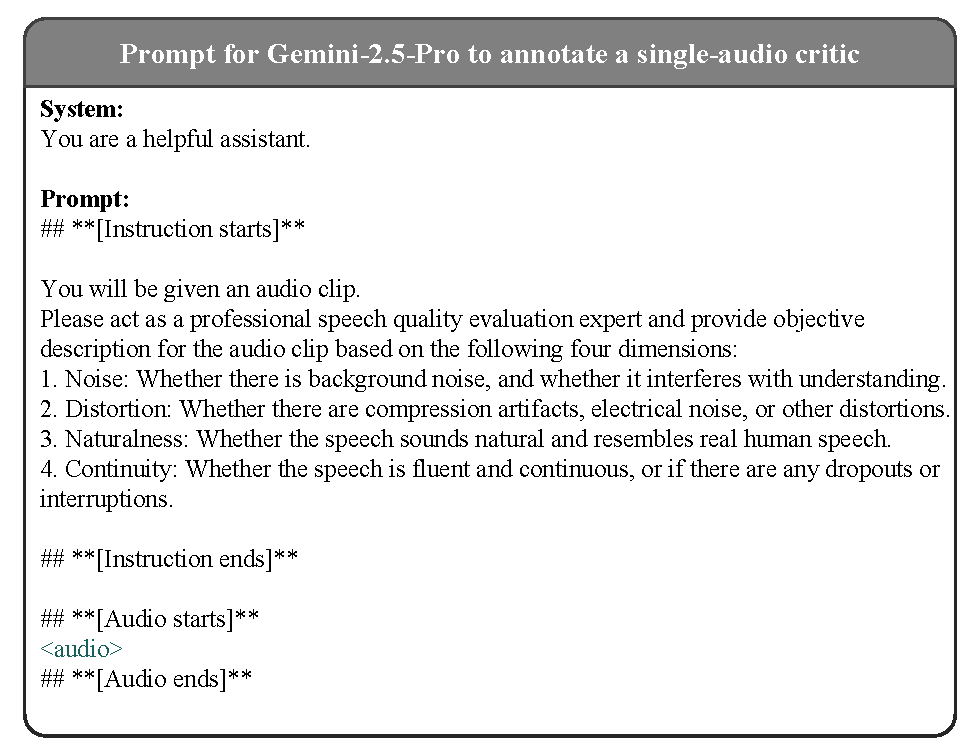
\includegraphics[width=\textwidth]{pictures/prompt-template/annotate-an-audio_crop.pdf}
\end{center}
\caption{Prompt structure for Gemini-2.5-Pro to annotate a single-audio critic.}
\label{fig:prompt:annotate-an-audio}
\end{figure}

\begin{figure}[tbh]
\setlength{\abovecaptionskip}{-2pt}
\begin{center}
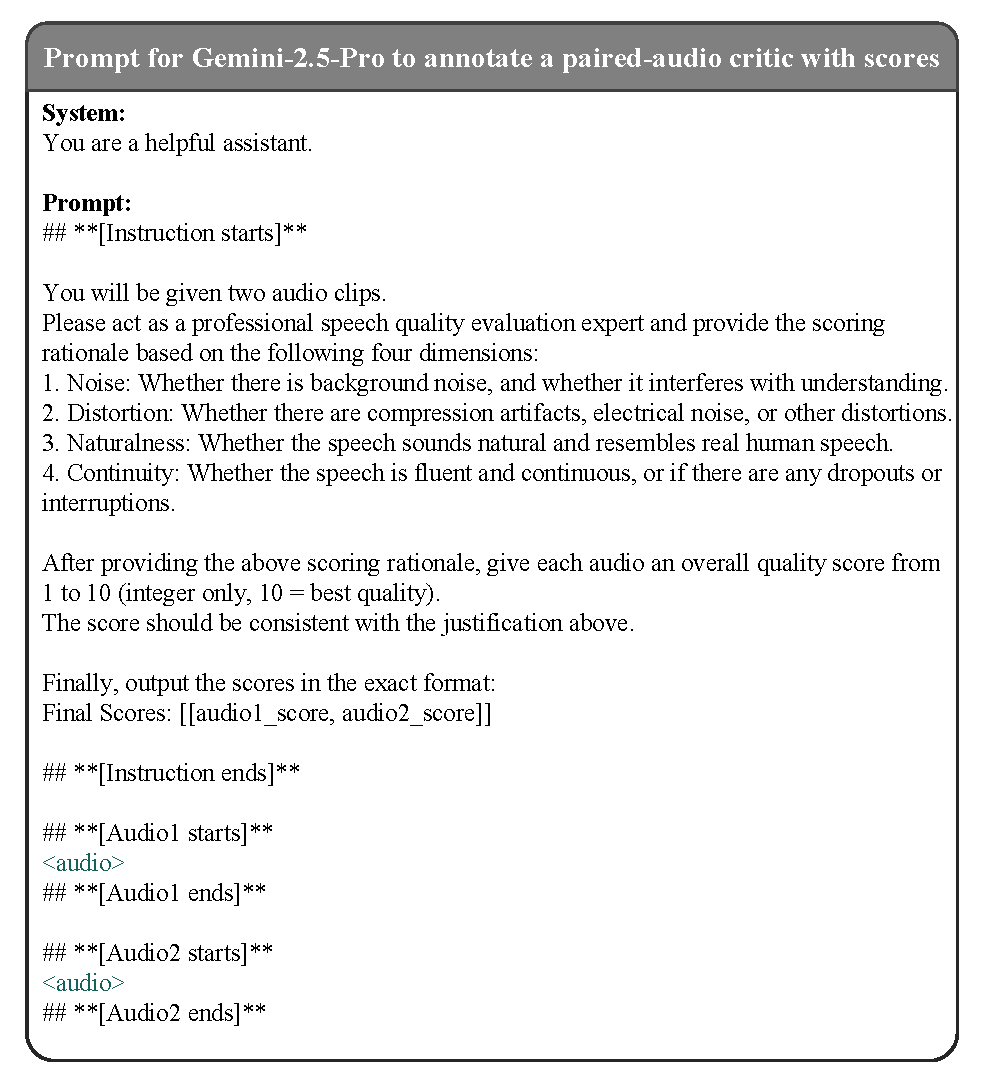
\includegraphics[width=\textwidth]{pictures/prompt-template/annotate-two-audios_crop.pdf}
\end{center}
\caption{Prompt structure for Gemini-2.5-Pro to annotate a paired-audio critic with scores.}
\label{fig:prompt:annotate-two-audios}
\end{figure}

\begin{figure}[tbh]
\setlength{\abovecaptionskip}{-2pt}
\begin{center}
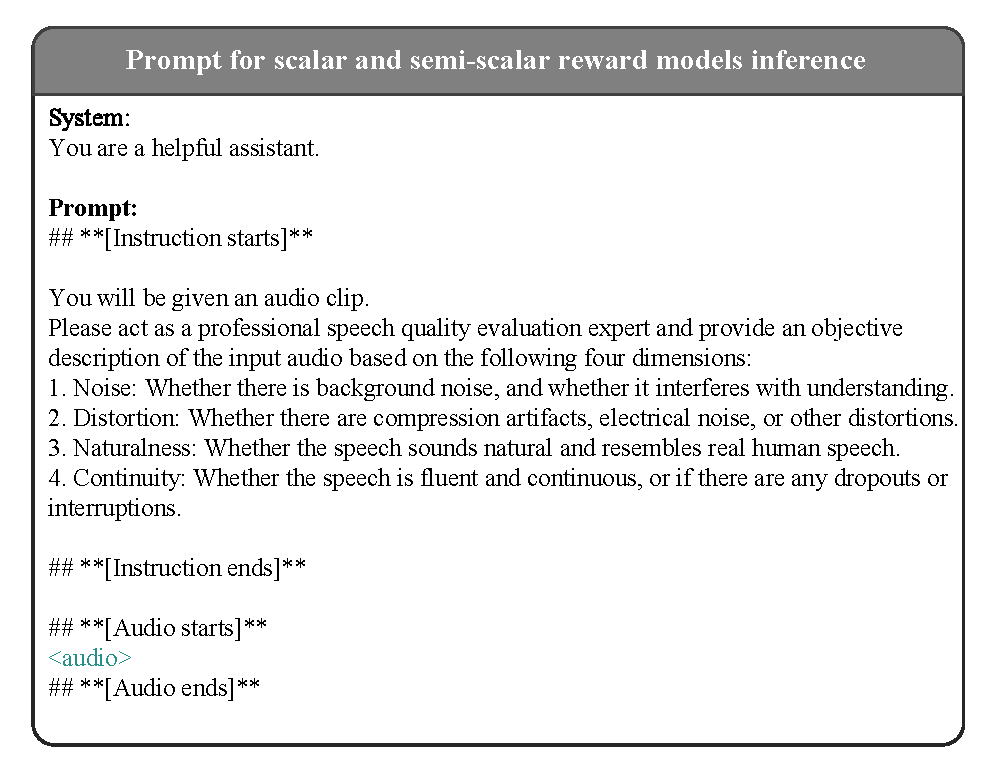
\includegraphics[width=\textwidth]{pictures/prompt-template/scalar-infer_crop.pdf}
\end{center}
\caption{Prompt structure for scalar and semi-scalar reward models inference.}
\label{fig:prompt:scalar-infer}
\end{figure}


\begin{figure}[tbh]
\setlength{\abovecaptionskip}{-2pt}
\begin{center}
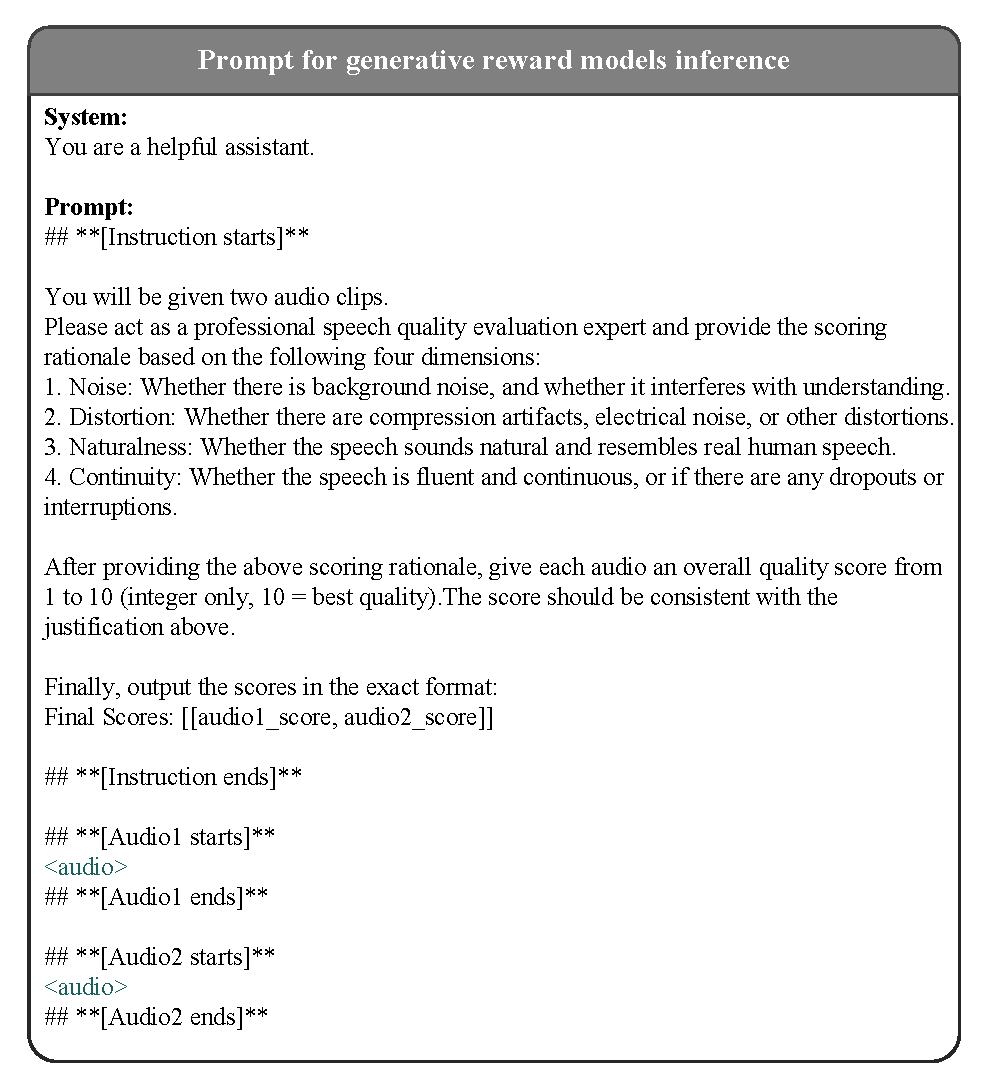
\includegraphics[width=\textwidth]{pictures/prompt-template/GRM-infer_crop.pdf}
\end{center}
\caption{Prompt structure for generative reward models inference.}
\label{fig:prompt:GRM-infer}
\end{figure}

\begin{figure}[tbh]
\setlength{\abovecaptionskip}{-2pt}
\begin{center}
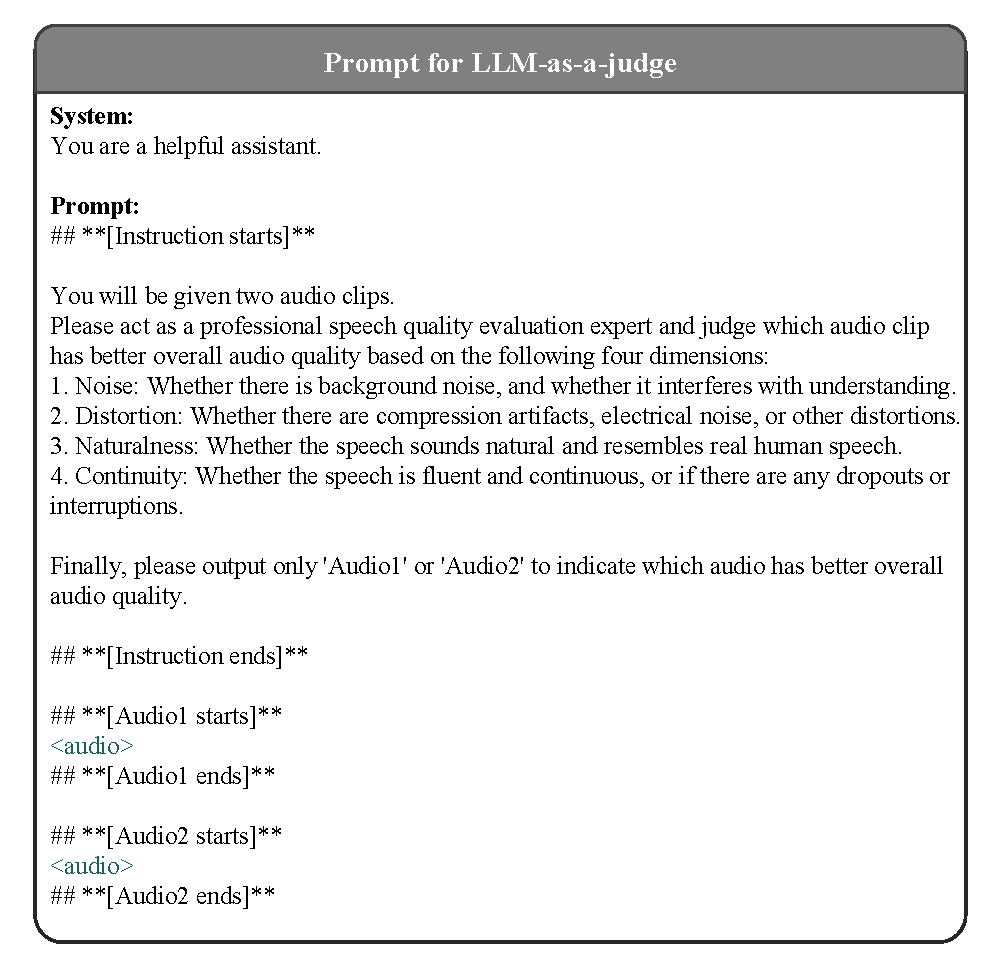
\includegraphics[width=\textwidth]{pictures/prompt-template/LLM-as-a-judge_crop.pdf}
\end{center}
\caption{Prompt structure for LLM-as-a-judge.}
\label{fig:prompt:llm-as-a-judge}
\end{figure}